\documentclass{acm_proc_article-sp}


\usepackage{listings}
\usepackage[T1]{fontenc}
\usepackage[utf8]{inputenc}
\usepackage{url}
%\usepackage{amsmath}
%\usepackage{amssymb}
\usepackage[usenames]{color}
\usepackage{graphicx}
\usepackage{xspace}% space in macros 
\usepackage{multirow}
\usepackage[font=bf,labelfont=bf]{caption}
% fixes caption package
\DeclareCaptionType{copyrightbox} 

\usepackage{subcaption}
\usepackage{tabularx}


% ----- begin macros
\lstdefinelanguage{Scala}%
{morekeywords={abstract,%
  case,catch,char,class,%
  def,else,extends,final,for,%
  if,import,implicit,%
  match,module,%
  new,null,%
  object,override,%
  package,private,protected,public,%
  for,public,return,super,%
  this,throw,trait,try,type,%
  val,var,%
  with,while,%
  yield%
  },%
  sensitive,%
  morecomment=[l]//,%
  morecomment=[s]{/*}{*/},%
  morestring=[b]",%
  morestring=[b]',%
  showstringspaces=false%
}[keywords,comments,strings]%

\lstset{language=Scala,%
  mathescape=true,%
%  columns=[c]fixed,%
%  basewidth={0.5em, 0.40em},%
  aboveskip=1pt,%\smallskipamount,
  belowskip=1pt,%\negsmallskipamount,
  lineskip=-0.2pt,
  basewidth={0.54em, 0.4em},%
  basicstyle=\ttfamily,%\scriptsize,%
  keywordstyle=\bfseries%\sffamily\bfseries,%
%  keywordstyle=\sffamily\bfseries,%
%  xleftmargin=0.5cm
}

\lstnewenvironment{listing}{\lstset{language=Scala}}{}
\newcommand{\scode}[1]{\lstinline[language=Scala,columns=fixed,basicstyle=\ttfamily]|#1|}
\newcommand{\jcode}[1]{\lstinline[language=Java,flexiblecolumns=true,basicstyle=\ttfamily]{#1}}
\newcommand{\code}[1]{\scode{#1}}

\newcommand{\todo}[1]{{\color{red} \textbf{[TODO: #1 ]}}}
\newcommand{\commentstyle}[1]{\slseries{#1}}
\newcommand{\keywordstyle}[1]{\bfseries{#1}}
\newcommand{\comment}[1]{}
\newcommand{\note}[1]{$\spadesuit$ \textbf{#1} $\clubsuit$}
\graphicspath{{figures/}}

\setlength{\floatsep}{2pt plus 2pt minus 2pt}
\setlength{\textfloatsep}{2pt plus 2pt minus 2pt}
\setlength{\intextsep}{2pt plus 2pt minus 2pt}
\setlength{\dblfloatsep}{2pt plus 2pt minus 2pt}
\setlength{\dbltextfloatsep}{2pt plus 2pt minus 2pt}
%\setlength{\bibsep}{0.0pt}

% Packed item, so we don't waste space
\newenvironment{sitemize}{
\begin{itemize}
  \setlength{\itemsep}{1pt}
  \setlength{\parskip}{0pt}
  \setlength{\parsep}{0pt}
}{\end{itemize}}
% ----- end macros

\raggedbottom


\newcommand{\tool}{Jet\xspace}
\newcommand{\coll}{DColl\xspace}
\newcommand{\NL}{\\}% \newcommand{\NL}{}
\newcommand{\PB}{\pagebreak} % \newcommand{\PB}{}

\begin{document}
  %\conferenceinfo{BigData'12,} {(date and location)}
  %\CopyrightYear{2012}
  %\copyrightdata{(provided by acm)}

  %
  % Title
  % 
    
  \title{\tool: An Embedded DSL for High Performance Big Data Processing}
  %\subtitle{[Extended Abstract]
  %\titlenote{A full version of this paper is available as
  %\textit{Author's Guide to Preparing ACM SIG Proceedings Using
  %\LaTeX$2_\epsilon$\ and BibTeX} at
  %\texttt{www.acm.org/eaddress.htm}} 


  %
  % Authors
  % 
  \numberofauthors{4} 
  \author{
	\alignauthor
	Stefan Ackermann\\
	 \affaddr{ETH Z\"urich}\\
	 \email{stefaack@student.ethz.ch}
     \alignauthor
    Vojin Jovanovi\'c\\
     \affaddr{EPFL, Switzerland}\\
	 \email{vojin.jovanovic@epfl.ch}
    \alignauthor
     Tiark Rompf\\
     \affaddr{EPFL, Switzerland}\\
	 \email{tiark.rompf@epfl.ch}
	 \and
     \alignauthor          
     Martin Odersky\\
     \affaddr{EPFL, Switzerland}\\
	 \email{martin.odersky@epfl.ch}         
% \and for another row of authors
  }
  
%  \additionalauthors{Additional authors: John Smith (The Th{\o}rv{\"a}ld Group,
%	email: {\texttt{jsmith@affiliation.org}}) and Julius P.~Kumquat
%	(The Kumquat Consortium, email: {\texttt{jpkumquat@consortium.net}}).}
  
  
  
  \date{31 August 2012}
  \maketitle
  
  \begin{abstract}
    Cluster computing systems today impose a trade-off between generality,
performance and productivity. Hadoop and Dryad force programmers to write low
level programs that are tedious to compose but easy to optimize. Systems like
Dryad/LINQ and Spark allow concise modeling of user programs but do not apply
relational optimizations. Pig and Hive restrict the language to achieve
relational optimizations, making complex programs hard to express without user
extensions. However, these extensions are cumbersome to write and disallow
program optimizations.

We present a distributed batch data processing framework called \tool.
\tool uses deep language embedding in Scala, multi-stage programming and
explicit side effect tracking to analyze the structure of user programs. The
analysis is used to apply projection insertion, which eliminates unused data, as
well as code motion and operation fusion to highly optimize the performance
critical path of the program. The language embedding and a high-level interface
allow \tool programs to be both expressive, resembling regular Scala code, and
optimized. Its modular design allows users to extend \tool with modules that
produce highly performant code. Through a modular code generation scheme, \tool
can generate programs for both Spark and Hadoop. Compared with na\"{\i}ve
implementations we achieve 143\% speedups on Spark and 126\% on Hadoop.

  \end{abstract}
  \category{H.2.3}{Database Management}{Languages}    
  \terms Languages, Performance
  \keywords Domain-specific Languages, Multi-stage Programming, MapReduce,
  Operation Fusion, Projection Insertion


  %
  % Sections 
  %
  \section{Introduction}
\label{sec:introduction}

% Motivation -- three different types programming models and their problems
In the past decade, numerous systems for big data cluster computing have been studied \cite{dean_mapreduce:_2008, yu_dryadlinq:_2008-1, olston_pig_2008-1, thusoo_hive_2010-1, spark-nsdi}. Programming models of these systems impose a trade-off between generality, performance and productivity. Systems like Hadoop MapReduce, \cite{hadoop} and Dryad \cite{isard_dryad:_2007} provide a low level general purpose programming model that allows writing fine grained and optimized code. However, low level optimizations greatly sacrifice productivity \cite{chambers_flumejava:_2010}. Restricted programming models like Pig latin \cite{olston_pig_2008-1} exploit domain knowledge to provide both good performance and productivity for a large number of use cases. However, they support generality only through user defined functions that are cumbersome and difficult to optimize. Finally, models like Spark \cite{spark-nsdi}, FlumeJava \cite{chambers_flumejava:_2010} and Dryad/LINQ \cite{yu_dryadlinq:_2008-1} provide high level operations and general purpose programming models, but their performance is limited by glue code between high level operations. Also, many relational optimizations are impossible due to the lack of knowledge about the program structure. 

% Trade-off - why cant there be both generality, performance and productivity
Above mentioned trade-off exists due to the imperative programming models, run-time binding of methods and open world assumptions commonly used in languages for big data processing. This limits compiler's ability to optimize the code. Inefficient abstractions like iterators and channels are not removed from the code that connects declarative operations. Side effect free operations like date/time instantiation, regular expression compilation and high precision decimal numbers are often hidden by abstraction and recomputed in the hot path for each piece of data. 

Domain specific approaches, like Pig and SQL, have a narrow and side effect free interface and provide good optimizations. However, they come with their own set of limitations. Their programming model is often too simple for the problem. This requires reverting to external language operations, which are again hard to optimize, or to abandoning the model completely. Moreover, there is the high overhead of learning the new language and proper tool support debugging, type driven correctness checking and IDE support is often limited. Also it is hard to extend these frameworks with optimizations for a new domain.

% Existing Solutions to achieve this
In the recent history there have been several solutions that try to make programming big data systems efficient, productive and general at the same time. Steno \cite{murray_steno:_2011} implements an innovative runtime code generation scheme that eliminates iterators in Dryad/LINQ queries. It operates over flat and nested queries and produces a minimal number of loops without any iterator calls. Manimal \cite{jahani_automatic_2011} and HadoopToSQL \cite{iu_hadooptosql:_2010} apply byte code analysis to extract information about unused data columns and selection conditions to gain enough knowledge to apply common relational database optimizations for projection and selection. However, since these solutions use static byte code analysis they must be safely conservative which can lead to missed optimization opportunities.

% general, restricted
% optimizations
% modular/extensible
% portable
This paper presents a new domain specific language \tool for big data processing that provides a high level declarative interface similar to Dryad/LINQ and Spark. \tool builds upon language virtualization \cite{moors_scala-virtualized_2012} and lightweight modular staging \cite{rompf_lightweight_2010} (LMS) and has the same syntax and semantics as the regular Scala language with only a few restrictions.
Because \tool includes common compiler and relational optimizations, as well as domain specific ones, it produces very fast programs. It is designed in a very modular way - the code generation is completely independent of the parsing and optimizations - and allows extensions for supported operations, optimizations and backends. 
% Our implementation

% Contributions
\tool makes following contributions to the state of the art:    
\begin{itemize}

  \item We implement the \tool framework for big data processing. \tool has a high level programming model with carefully chosen restrictions that allow relational, domain specific and compiler optimizations but do not sacrifice generality.
%  \item \todo{link generality to optimizations}We implement the \tool framework for big data processing. \tool has a slightly restricted and high level programming model but still applies relational, domain specific and compiler optimizations to achieve high performance.

  \item We introduce a novel projection insertion algorithm that operates across general program constructs like classes, conditionals, loops and user defined functions, takes the whole program into account and does not rely on safe assumptions which lead to missed optimization opportunities.  

  \item We show that \tool allows easy language extension and code portability for big data frameworks. 

\end{itemize} 

% Sections
In section \ref{sec:background} we will provide background on LMS, language virtualization and big data frameworks. Then, in section \ref{sec:programming-model} we explain the programming model and present simple program examples. In section \ref{sec:optimizations} we explain the novel projection insertion optimization algorithm in section \ref{sec:field-reduction} and section \ref{sec:fusion} explains the fusion optimization. We evaluate \tool in \ref{sec:evaluation} and discuss our approach in section \ref{sec:discussion}. \tool is compared to state of the art in section \ref{sec:related-work}, future work is in section \ref{sec:future-work} and we conclude in section \ref{sec:conclusion}.

  \section{Background}
\label{sec:background}

% language virtualization
\subsection{Virtualized Scala}
\label{subsec:virtualized-scala}
\tool is written in an experimental version of Scala called Virtualized Scala \cite{sv}. Virtualized Scala provides facilities for simplified deep embedding of domain specific languages. Main facility for achieving this is the desugaring of regular language constructs like conditionals, loops, variable declarations, return statements and equality comparisons to simple method calls. For example, \code{if (c) a else b} gets translated to an \code{__ifThenElse(c, a, b)} method call. In the case of regular language execution this method executes the logic of the conditional but in case of deeply embedded DSLs it is used for creation of  IR node that represents the \code{if} statement.  

In Virtualized Scala, all embedded DSLs are written within DSL scopes. These special scopes look like method invocations that take one by name parameter. However, they get translated to the complete specification of DSL modules that are used in a form of a Scala trait mix-in composition\todo{put a star what is a mixin composition}. For example: 
\code{stivo\{ \\\\ dsl code \}} gets translated into:
\scode{new StivoDSL \{
 def main()\{
   \\\\ dsl code
 \}
\}} 
This makes all the DSL functionality defined in StivoDSL visible in body of the by name parameter passed to stivo method. 
Although modified, Virtualized Scala is fully binary compatible with Scala and can use all existing libraries.  

  
%??? infix-methods, if the type of expression x does not have method m but there is an infix method defined in the scope it will be desugared to infix_m(x) of the expression x m does not type check 

\subsection{Lightweight Modular Staging}
\label{subsec:lightweight-modular-staging}

% lms basics 
The base for the \tool project is LMS (Lightweight Modular Staging) library \todo{cite}. It utilizes facilities provided by Virtualized Scala to build a modular infrastructure for developing staged DSLs. LMS library represents types in a DSLs with an polymorphic abstract data type \code{Rep[T]}. When in a DSL scope term has type \code{Rep[T]} it means that once the code is staged, optimized and generated the actual result of the term will have type \code{T}.  Since \code{Rep[T]} is and abstract type each DSL module can specify concrete operations on it which are used for simple building of the DSL intermediate representation. For example: 

% Here we represent a simple Exp example in several lines of code.
 
Since Scala's type system supports type inference \todo{which? It is not HM.} most of the Rep[T] types are hidden from the DSL user. This makes the DSL code almost completely free of type information and makes the user almost unaware of the Rep types. The only exception for visibility of Rep types are the parameters of defined methods and fields of defined classes. In our experience with writing DSLs, Rep types do not present a problem but gathering precise and unbiased information is very difficult. 

% LMS effects
Unlike Scala, which does not have an official effects tracking mechanism, LMS expects the DSL developer to explicitly specify exact effects for each DSL operation. LMS effect tracking system than calculates the effects summary for each basic block in the code. This allows the optimizer to apply code motion operations on th e pure parts of the code and remove constant expressions out of hot loops as well as push expressions inside conditionals. The framework provides effects tracking for numerical operations and all basic language constructs, but all other effects are up to the DSL developer. Although, it is hard for the DSL developer to specify effects for each operation the overall performance gain is large. Also, due to LMS modularity the effects for most commonly used facilities like strings, arrays, loops and conditionals are 100\% reusable.


% modularity through scalable components abstraction.
Modular design of LMS allows the DSL developer to arbitrary compose the interface, optimizations and code generation of the DSL. Since LMS provides modules for large part of the Scala language and most common libraries if the DSL developer decides to include all the modules, the language will be very general and similar to the native Scala language. Module inclusion is simply done by mixing in Scala traits together. The correctness of the composition are checked by the type system and missing dependencies are caught by the type checking system. Code generation for a DSL is also modular so actual module for a single DSL is usually very thin since it reuses other modules in the library.
  \section{Programming Model}
\label{sec:programming-model}

% Scala and Spark and Collections like interface
The basic abstraction in our programming model is the interface \scode{DList[T]}. \scode{DList[T]} represents a distributed collection of elements that have type \scode{S} which is the subtype of \scode{T}. The elements of the \scode{DList[T]} collection are immutable so each operation on the list can only: \emph{i)} produce a new \scode{DList}, \emph{ii)} save it to persistent storage, \emph{iii)} materialize it on the master node or \emph{iv)} return an aggregate value. 

% Operations and reference to the table. monadic operations, concat, partitionBy, cache, count returns the value
\code{DList} operations are presented in Table \ref{tbl:operations}. In the left column we show which frameworks support which method, the middle column shows the method name and the right column contains the type of the \code{DList} that the operation is called on and the return type. 

Operations \code{DList} and \code{save} are used for loading and storing data to the persistent storage. \code{map, filter} and \code{flatMap} are standard list comprehensions for transforming the data by applying the argument function and can also be used with Scala \code{for} comprehensions. Operations \code{groupByKey}, \code{join}, \code{cogroup}, \code{cross} and \code{reduce} are applicable only if the elements of \code{DList} form a key/value tuple. \code{reduce} is used for general aggregation after the \code{groupByKey}, \code{join, cogroup} and \code{cross} are different types of relational joins. \code{sort} sorts the dataset, \code{partitionBy} defines partitioning among machines and \code{cache} signals that data should be kept in cluster memory for faster future accesses. Two \code{DList}s can be concatenated by operation \code{++}.

Some methods accept functions as their parameters. Code within these functions can be either written in \tool DSL or by using existing functions from user or common JVM libraries. Using JVM libraries requires just one extra line of code per method.  

\begin{table*}
\centering
\begin{tabular}{|c|l|l|} \hline
Framework  & Operation & Transformation\\ \hline

\multirow{12}{*}{All}		       		& \scode{DList(uri: Rep[String])}      				& \scode{String => DList[T]}\\ %\cline{2-3}
								& \scode{save(uri: Rep[String])}      				        & \scode{DList[T] => Unit}\\ %\cline{2-3}
								& \scode{map(f: Rep[T] => Rep[U])}      				& \scode{DList[T] => DList[U]}\\ %\cline{2-3}
								& \scode{filter(f: Rep[T] => Rep[Boolean])}			& \scode{DList[T] => DList[T]}\\ %\cline{2-3}
								& \scode{flatMap(f: Rep[T] => Rep[Iter[U]])}		        & \scode{DList[T] => DList[U]}\\ %\cline{2-3}
								& \scode{groupByKey()} 							& \scode{DList[(K, V)] => DList[(K, Iter[V])]}\\ %\cline{2-3} 
								& \scode{reduce(f: (Rep[V], Rep[V]) => Rep[V])} 	        & \scode{DList[(K, Iter[V])] => DList[(K, V)]}\\ %\cline{2-3} 
								& \scode{cogroup(right: Rep[DList[(K, W)]])} 			& \scode{DList[(K, V)] => DList[(K, (Iter[K], Iter[W]))]}\\ %\cline{2-3} 								
								& \scode{join(right: Rep[DList[(K, W)]])} 			& \scode{DList[(K, V)] => DList[(K, (V, W))]}\\ %\cline{2-3} 
								& \scode{++(other: Rep[DList[T]])}		                & \scode{DList[T] => DList[T]]}\\ %%\cline{2-3}							
								& \scode{partitionBy(p: Rep[Partitioner[T]])} 			& \scode{DList[T] => DList[T]}\\ %\cline{2-3} 
								& \scode{takeSample(p: Rep[Double])} 					& \scode{DList[T] => Seq[T]}\\ \hline
\multirow{2}{*}{Spark}			        & \scode{cache()} 								& \scode{DList[T] => DList[T]}\\ %\cline{2-3} 
								& \scode{sort(cmp: Rep[Comparator[T]])}			& \scode{DList[T] => DList[T]}\\ \hline
Crunch						        & \scode{sort(asc: Rep[Boolean])}					& \scode{DList[T] => DList[T]} \\ \hline
\end{tabular}
\caption{DList operations and their framework support. For clarity reasons, \scode{Iter} represents the Scala \scode{Iterable} and \scode{Rep[_]} types in the rightmost column are omitted.  }
\label{tbl:operations}
\end{table*}

% Example word count application
In the listing \ref{lst:wordcount} we show an implementation of a simple word count example, in which the code does not have visible \code{Rep} types. Since a large subset of the Scala library is implemented as a DSL module, functions like \code{split} and string concatenation are used the same way as they are in Scala. In the second line the regular (with arguments wrapped in \code{Rep}) method \code{parse} is passed to the \code{map} method. Pig and Hive do not have functions in their own language, but allow writing user defined functions in other languages which requires a noticeable amount of boilerplate code.

% Word count showing generality, rep clean api.
\begin{lstlisting}[name=code, caption=Example of word count program where type inference removes the need to declare any \scode{Rep} types., captionpos=b, label=lst:wordcount, float=t]
    val read = DList("hdfs://..." + input)
    val parsed = read.map(WikiArticle.parse(_))
    parsed.flatMap(_.split("\\s"))
      .map(x => (x, 1))
      .groupByKey
      .reduce(_ + _)
      .save("hdfs://..." + output)
\end{lstlisting}

All methods except for \code{cache} and \code{sort} can be mapped to methods in Scoobi, Spark and Crunch. We have checked that other back-ends (including Dryad) provide these primitives as well. Method \code{cache} currently works with Spark only but it can be added to the interface of other back-ends without any effect, such that the code stays portable. From existing frameworks today only HaLoop\cite{bu_haloop:_2010} and Twister \cite{ekanayake_twister:_2010} can benefit from it, however we did not implement code generation for them. Method \code{sort} is inconsistent in most of the frameworks so we have not mapped uniformly to all of them. However, with slight modifications to the framework implementations it could be supported as well. \code{sort} can also be implemented in \tool itself by using \code{takeSample} and \code{partitionBy}.
  \section{Optimizations}
\label{sec:optimizations}
In this section we present the main optimizations implemented in \tool.
\subsection{Projection Insertion}
\label{sec:field-reduction}

% Intro/Motivation 
A common optimization in data processing is to early remove intermediate values that are not needed in later phases of the computation. It has been implemented in relational databases for a long time, and has recently been added to the Pig framework. This optimization requires all field accesses in the program to be explicit. A library can provide this, but the usage is more intrusive than if the framework can use compiler support. 

% description of supported types
In \tool we support this optimization for algebraic data types, more specifically final immutable Scala classes with a finite level of nesting. Our approach does not require special syntax or access operators and supports method declarations on a data type like regular Scala classes do. While implementing our benchmarks we found this to be a reasonably expressive model for big data programming. The DSL user needs to supply class declarations, from which we generate all the necessary code for its use in \tool. For these types, LMS describes all field accesses explicitly and we can generate highly specialized code for these types including serialization schemes and other glue code for the back-ends we support.


%\todo{Drop this sentence?}The generated code includes a parsing method, to which the user simply supplies a regular expression, in case the data is stored in text form. 

% explaining the lingo and high level overview of the algorithm.
In section \ref{subsec:lms-optimizations} we have shown how LMS optimizes these classes within the same program scope. However, in \tool we endorse a declarative programming model with many short functions - each having its own scope - as these are easier to read. Each operation in our API has an input type and an output type, and they may have a parameter accepting a closure. Operations are chained together to form a data flow graph without cycles. Since types support nesting, we need to define the live values between operations as the sequence of field dereferences respective to a type to access that value. This sequence of field dereferences we call a path, and to represent it we use the scala expression needed to access it on such a type. In figure \ref{fig:type_tree} we visualize the tree which contains all paths and fields for the nested type of t in the example code in \ref{lst:types}.

For our projection insertion algorithm we need to analyze the paths on each edge of the data flow graph. We can only compute the paths for one operation when the union of all paths accessed by its successors has been already computed. For this reason we visit the graph in reverse topologically sorted order and process the operations one by one. When the successors of a node have all been processed and their paths have been propagated, that node can be analyzed to compile a list of paths it needs from its predecessors. The result of this analysis can then be used to insert projections before any operation which serializes objects or stores them in memory - we call them barriers - for example \code{cache}, \code{groupByKey} or \code{join}.

\begin{figure}
% \begin{subfigure}
\begin{lstlisting}[name=code, caption=Nested type for paths example., captionpos=b, label=lst:types]
case class A(id: String, b: B)
case class B(id: String)  
val t = ("tuple", A("a", B("b"))) 
t: scala.Tuple2[String, A]
\end{lstlisting}
% \end{subfigure}
% \begin{subfigure}
\centering
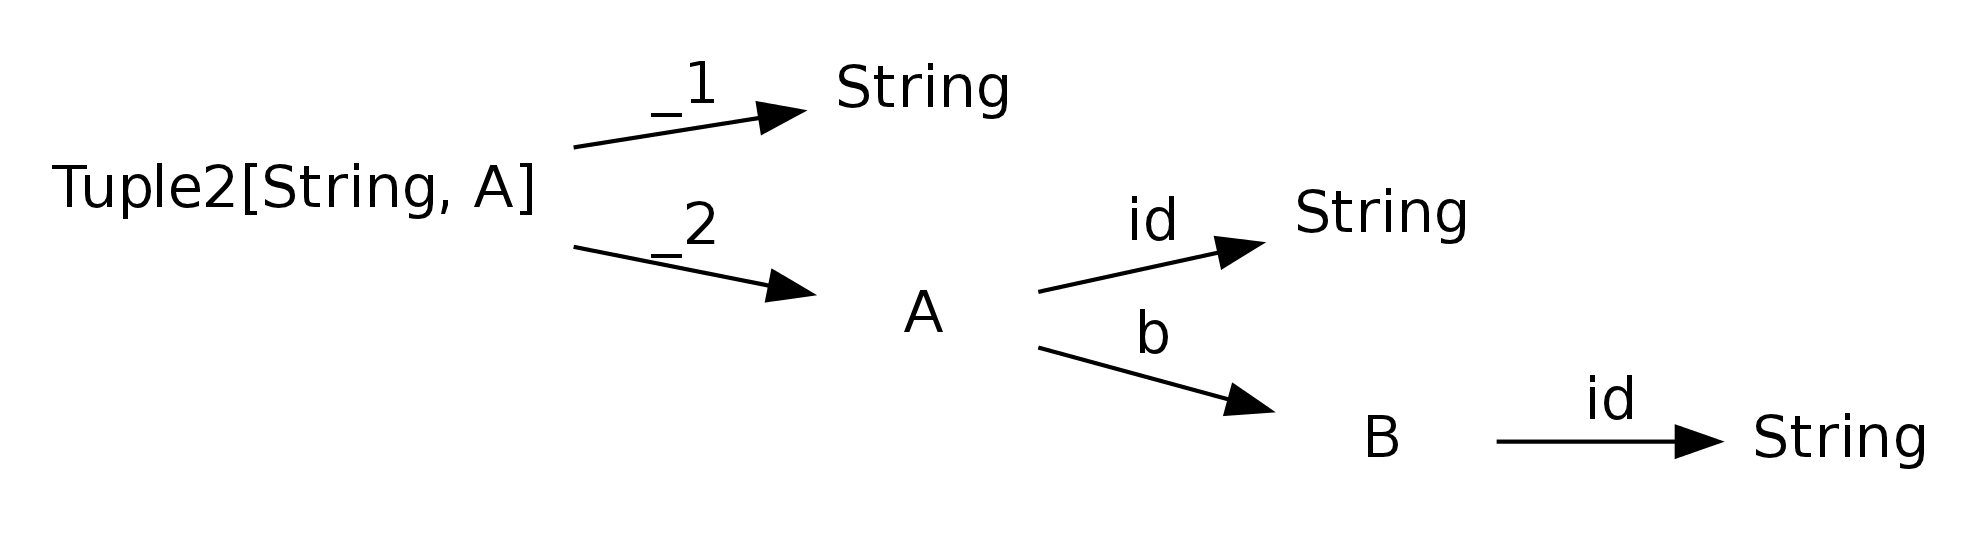
\includegraphics[clip=true, width=0.95\columnwidth]{dot/access.png}
\caption{Visualization of the nested type Tuple2[String, A]. The node labels are the types at that path, the edges describe one field dereference. The leafs are always primitive types, and the path to them is formed by concatenating the edge labels. An example path description is ``\_2.b.id''}
\label{fig:type_tree}
% \end{subfigure}
\end{figure}

% explaining the analysis

The algorithm depends on the analysis of a single operation, which we implemented using following primitives:
\begin{itemize}
\item \emph{Paths for type}: Given a type and optionally a path, this primitive creates paths for all the nested fields within. In \ref{lst:types} a \code{save} with element type A returns the paths \code{id} and \code{b.id}. 
\item \emph{Closure analysis}: This primitive returns a list of all paths accessed in a closure that read (recursively) from the closure's input.
\item \emph{Rewrite paths}: Several operations have defined semantics which influence the type and therefore the paths. For example, the \code{cache} operation will always have the same input and output type and is known to return the same instance, so all paths from it's successors must be propagated to its predecessors. The \code{groupByKey} operation on the other hand always reads all parts of the key, and has to rewrite all paths of the form \code{\_2.iterable.x} to \code{\_2.x}, as the iterable is introduced by the operation itself and is known to conserve the instances.
\item \emph{Narrow closure}: Given a list accessed paths and a closure, this primitive replaces the closure's original output symbol with one that reads from it and creates a new object only containing the fields needed for later stages.
\end{itemize}

For \code{map} operations which output a nested type we need to combine the narrow closure and the closure analysis primitive. SOA ensures that the output symbol of a closure is always a constructor invocation for these. We then use the narrow closure primitive to create a new closure, in which the output symbol reads from the old output symbol. LMS recognizes a field read that reads from a constructor invocation in the same scope and optimizes this by reading the value that was used to initialize the field directly. This happens for all the fields, if the corresponding constructor invocation is in the same scope. Therefore the old constructor invocation will not be read anymore, and DCE will pick it up. This means that the field values only it was reading will also not be read anymore, and they too will be eliminated. Then we can analyze this new closure to get the accessed paths from it. 

Table \ref{table:field_reduction} shows how these primitives are combined to form the rules for the most important operations in our API.

 \begin{table}[width=0.5\pagewidth]

    \begin{tabularx}{0.5\textwidth}{l|X|l}
        operation    & Propagate accessed paths 							     & barrier \\ \hline
        filter       & All of successor + closure reads                                                      & ~       \\ 
        flatMap      & All of the closure with a replaced output                                             & ~       \\ 
        map          & All of the closure with a replaced output                                             & ~       \\ 
        join         & All paths for the key, rewrites accesses to values to the correct predecessor         & x       \\ 
        groupByKey   & All paths for the key, rewrites accesses to the value's iterable to the value itself  & x       \\ 
        reduce       & All accesses from the closure are translated to access of the value's iterable        & ~       \\ 
        save         & All paths for input type           	                                             & ~       \\ 
    \end{tabularx}
    
    \caption{Access path computation and propagation for selected operations.}
\label{table:field_reduction}
 \end{table}


  \subsection{Operation Fusion}
\label{sec:fusion}

In Section \ref{sec:programming-model} we have shown that the \code{DList} provides declarative higher order operations. Closures passed to these operations do not share the same scope of variables. This reduces the number of opportunities for the optimizations described in Section \ref{subsec:lms-optimizations}. Moreover, each data record needs to be read, passed to and returned from the closure. In both the push and the pull data flow model this enforces expensive virtual method calls \cite{murray_steno:_2011} for each data record. To reduce the performance penalty we have implemented fusion of operations \code{map}, \code{flatMap} and \code{filter} through the underlying loop fusion algorithm described in Section \ref{subsec:lms-optimizations}. 

The loop fusion optimization described in Section \ref{subsec:lms-optimizations} supports horizontal and vertical fusion of loops as well as fusion of nested loops. Also, it provides a very simple interface to the DSL developer for specifying loop dependencies and for writing fusible loops. We decided to extend the existing mechanism to the \code{DList} operations although they are not strictly loops. We could have taken the path of Murray et al. in project Steno \cite{murray_steno:_2011} by generating an intermediate language which can be used for simple fusion and code generation. Also, we could use the Coutts et al. \cite{coutts_stream_2007} approach of converting \code{DList} to streams and applying equational transformation to remove intermediate results. After implementing the algorithm by reusing loop fusion we are confident that it required significantly less effort than reimplementing existing approaches.

\begin{figure}[!ht]
We define the set of program \code{DList} nodes as $D$.\\
For $in \in D$:\\
 $pred(n)$ gives the predecessor of the node in $D$\\
 $succ(n)$ returns a set of node successors in $D$\\
 $prevent\_fusion(n) =  |succ(pred(n))| > 1$\\

\begin{lstlisting}
Transformation:

$out = map(in, op) \rightarrow  $
  $loop(shape\_dep(in, prevent\_fusion(in)), i, \{$
    $yield(out, op(iterator\_value(in))\\$
  $\})$
$out = filter(map, op) \rightarrow$
  $loop(shape\_dep(in, prevent\_fusion(in)), i, \{$
     $if (op(iterator\_value(in))$
       $yield(out, iterator\_value(in)) $
  $\})$
$out = flatMap(in, op) \rightarrow$
  $loop(shape\_dep(in, prevent\_fusion(in)), i, \{$
    $w = op(iterator\_value(in))$
    $loop(w.size, i, \{yield(out, w(i))\})$
  $\})$
\end{lstlisting}
\label{lst:lowering}
\caption{Operation lowering transformations.}
\end{figure}

Before the fusion optimization, the program IR represents an almost one to one mapping to the operations in the programming model. Each operation is represented by the corresponding IR node which carries its data and control dependencies and has one predecessor and one or more successors. On these IR nodes we first apply a lowering transformation, which translates operations \code{map}, \code{flatMap} and \code{filter} to an equivalent loop based representation. Described transformation is achieved by the program translation described in Listing \ref{lst:lowering}. These rules introduce two new IR nodes: \emph{i)} $shape\_dep(n, m)$ that carries the explicit information about its vertical predecessor and a $prevent\_fusion$ bit, and \emph{ii)} \code{$iterator\_value$} that represents reading from an iterator of the preceding \code{DList}. $shape\_dep$ stands in the place of the shape variable (eg. in.size) of the loop IR node. The \emph{yield} operation represents storing to the successor collection and is used in the LMS fusion algorithm for correct merging of two loops.

For the back-end frameworks that \tool supports, the fusion operation is not possible for all operations in the data flow graph. If one node has multiple successors, after fusion, it would form a loop that yields values to multiple \code{DList}s. This would be possible for Hadoop, as it supports multiple outputs in the \code{Map} phase but for Spark, Scoobi and Crunch is not feasible. To prevent fusion of such loops we added the $prevent\_fusion$ bit to the $shape\_dep$ node. We also prevent horizontal fusion by making $shape\_dep$ nodes always different in comparison.  

After the lowering transformation we apply the loop fusion optimization from LMS. It vertically fuses pairs of loops that do not have the $prevent\_fusion$ bit set until a fixed point is reached. In each fusion iteration all other LMS optimizations are applied as well. To avoid generating actual \code{while} loops we include a added a loop generation module for every back-end we support. This module emits the most general operation (equivalent of the Hadoop \code{Mapper} class) that the framework provides. With this approach we could also generate code directly for Hadoop MapReduce which would result in a single highly optimized loop per \code{Mapper}. After prototype experiments we concluded that the gain is not significant compared to using higher level back-ends. Therefore, as an alternative, we used the frameworks Scoobi and Crunch.

Unlike MapReduce based back-ends, Spark's design uses the pull data-flow model, implemented through iterators. Generating code for the pull data-flow model from the loop based model (push data-flow) proved to be non-trivial. After evaluating different types of queues and array buffers we have decided to buffer intermediate results in a 4 MB array.
  \section{Evaluation}
\label{sec:evaluation}

We evaluate \tool by implementing a word count program with prior text parsing, TPCH query 12 and a k-means application that uses array processing extension for \tool. \\

All experiments were performed on the Amazon EC2 Cloud, using 20 "m1.large" nodes as slaves and one as master. They each have 7.5 Gb of memory, 2 virtual cores with 2 EC2 compute units each, have 850 Gb of instance storage and provide high throughput. Prior to the experiments we have measured up to 50 MB/s between two nodes. For the Hadoop experiments we used current Clouderas Hadoop distribution cdh3u4. We used Crunch version 0.2.4 and Scoobi 0.4.0. We did not tweak Hadoop configuration beyond the default settings. For benchmarking Spark we used the Mesos \cite{hindman_mesos:_2011} EC2 script to start a cluster, and then most recent version of Spark for our tests.  For Spark we changed the default parallelism level to the number of machines in the cluster and increased the available memory to 6GB. 

% Regular expressions
For a fairer comparison with Pig we adapted some of their regular expression optimizations for our program. Pig makes use of a faster library \todo{cite brics.automaton} and implements an optimized splitting function when the regular expression becomes a simple comparison of one character. We implemented a frontend for regular expressions which automatically selects the best variant for each expression and operation. 

We were also getting unsatisfying numbers from our Scoobi backend, so we added Crunch with about one week of effort. This really shows that it is easy to implement a new backend, and the modularity allows us to reuse pieces of other backends. Crunch's implementation of join performed very badly in local benchmarks, so we replaced it with our own one for these benchmarks.

% Data Serialization
For serialization of data we used LMS code generation to achieve minimal overhead for both Crunch and Scoobi frameworks. We used generated versions since they outperformed the Kryo framework by a thin margin. For Spark we used Kryo. All benchmarks were run three times and in the figures we present only the average. We also measured standard deviation but it is not displayed since it is smaller than 3\% of the job time in all experiments.

\begin{figure}[!hbt]
    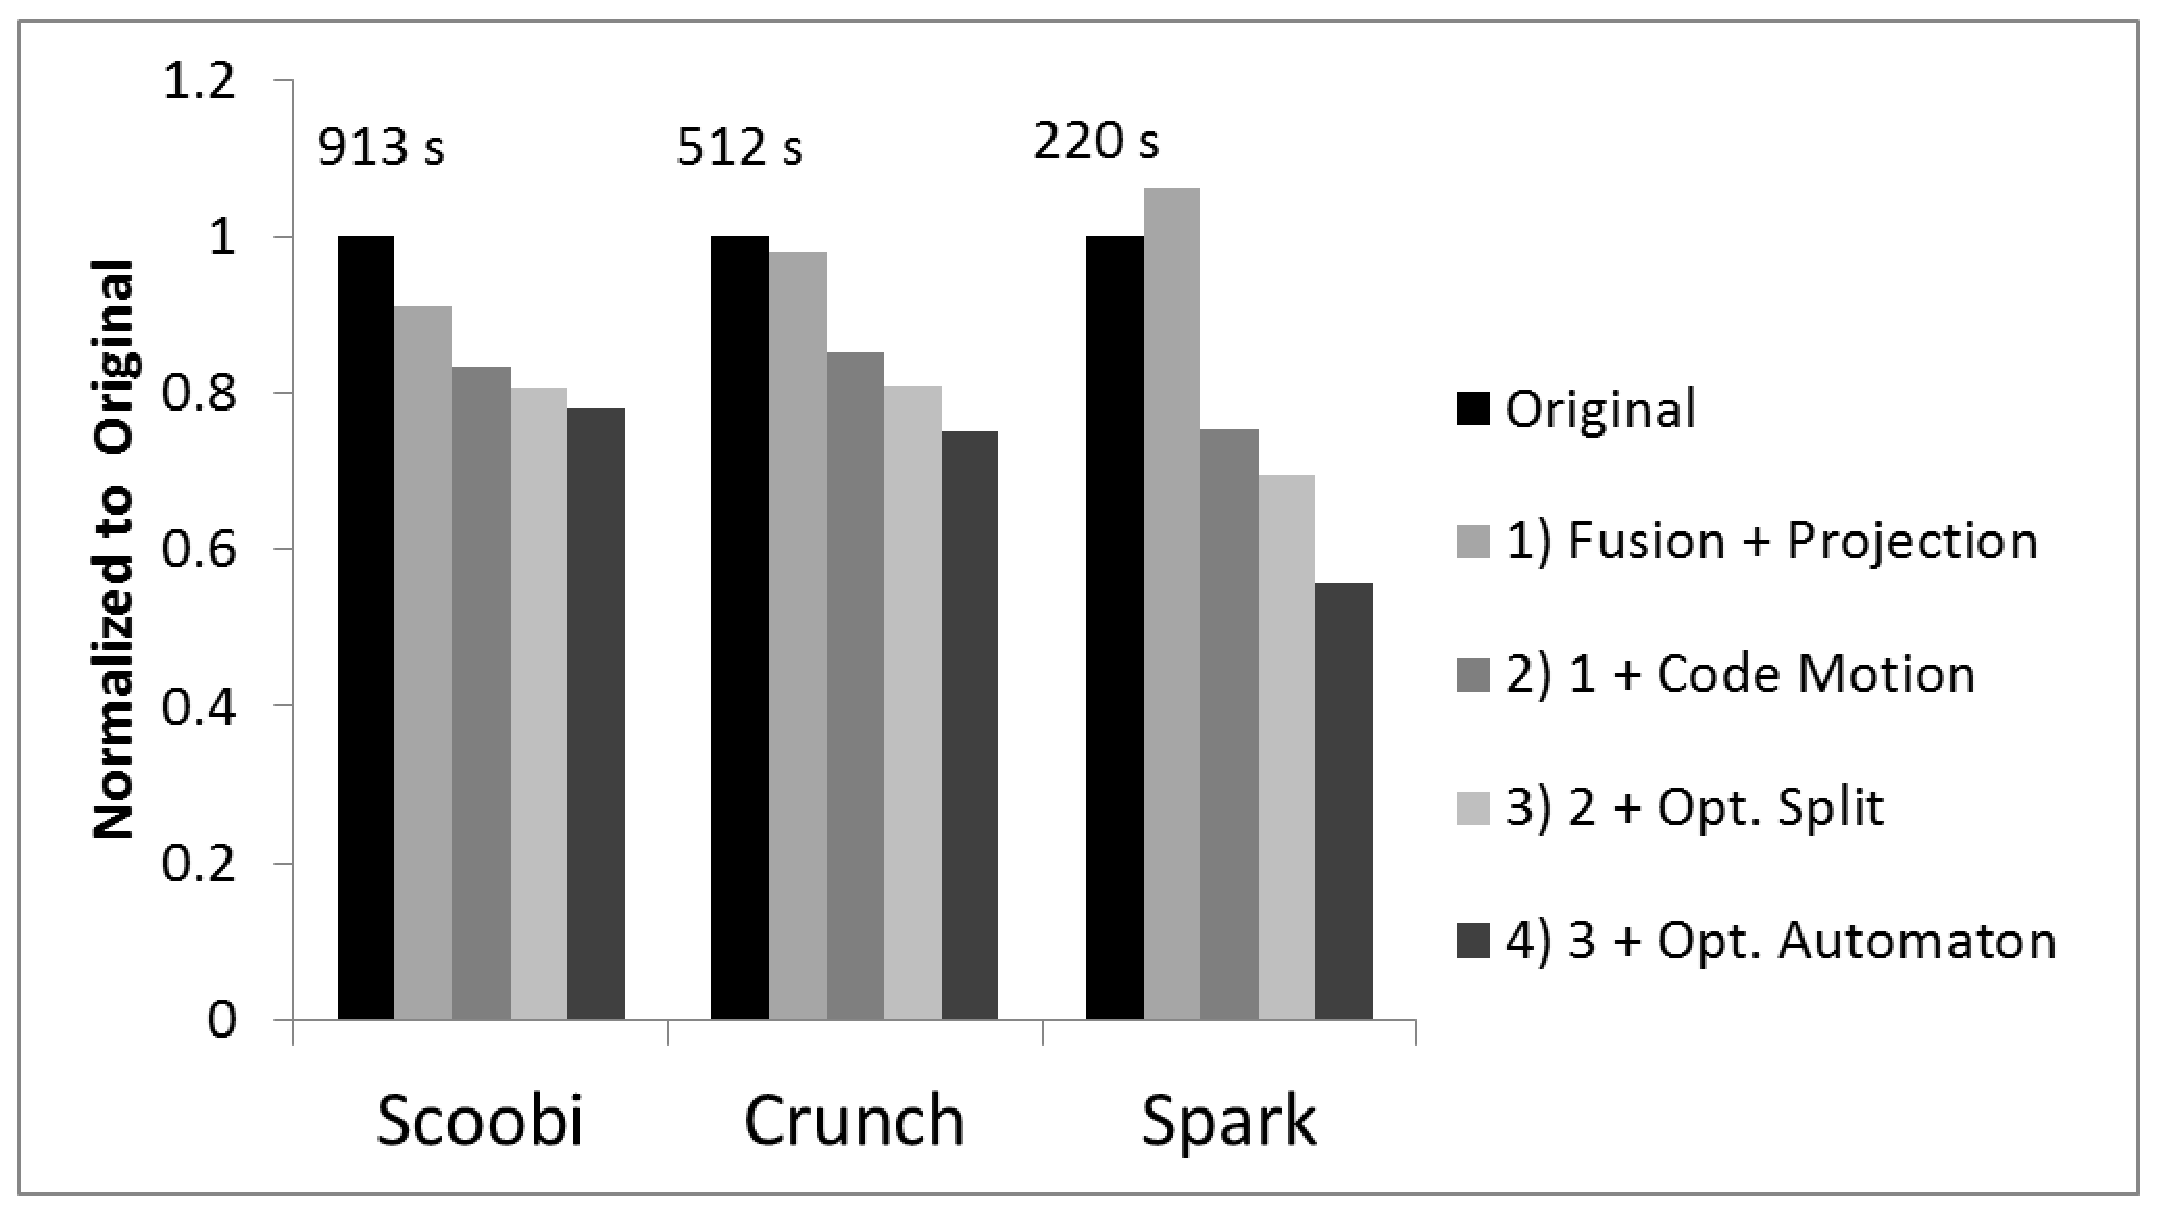
\includegraphics[width=8.6cm]{figures/word-count}
    \label{fig:word-count}\\%\vspace{10pt}
   \caption{Word Count benchmark.}
\end{figure}

\begin{figure}[!hbt]
    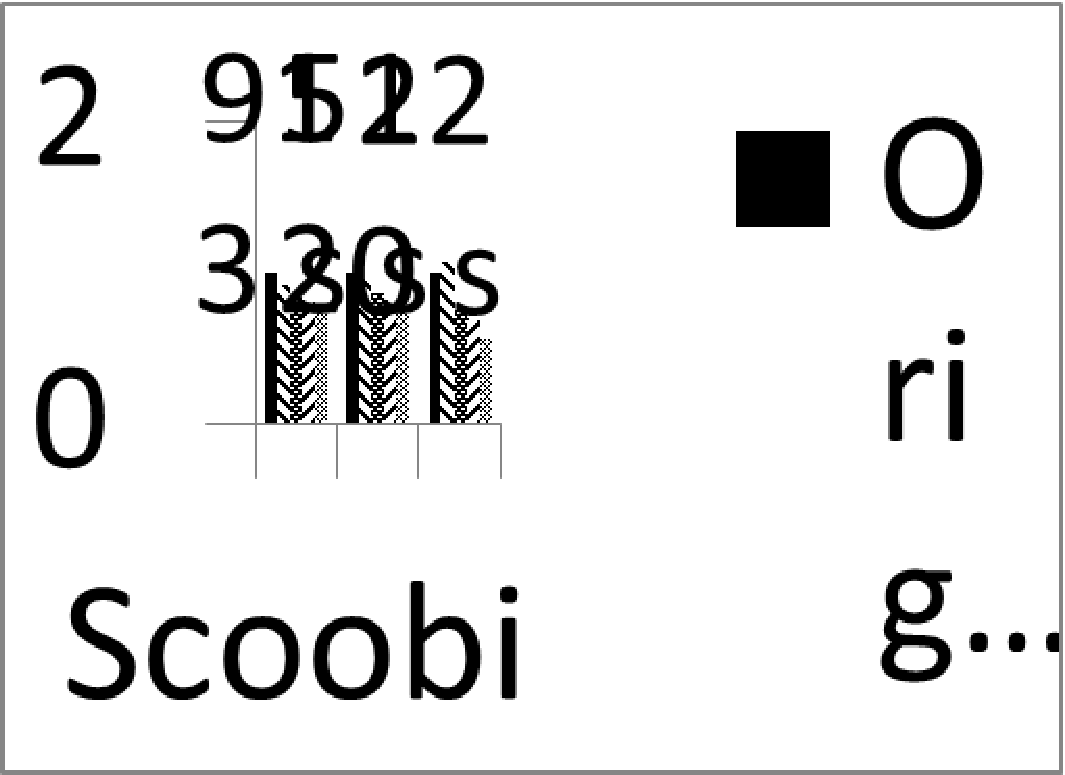
\includegraphics[width=8.6cm]{figures/k-means}
    \label{fig:k-means}\\%\vspace{10pt}
   \caption{K-means benchmark.}
\end{figure}

\begin{figure}[!hbt]
    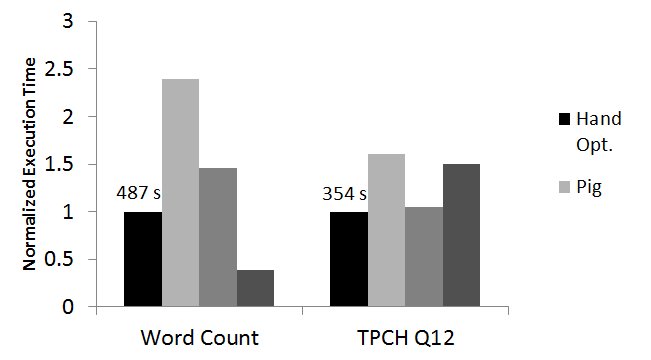
\includegraphics[width=8.6cm]{figures/pig}
    \label{fig:pig}\\%\vspace{10pt}
   \caption{Comparison with Pig.}
\end{figure}

\begin{figure}[!hbt]
    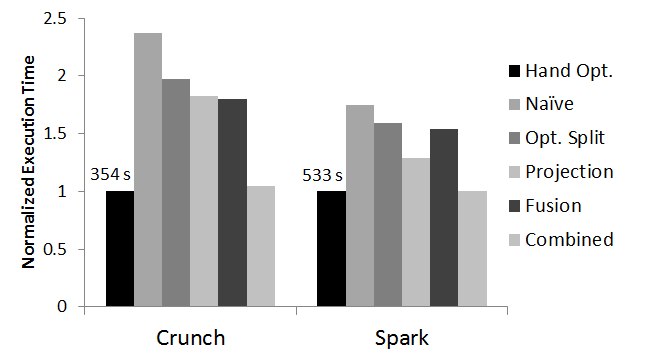
\includegraphics[width=8.6cm]{figures/tpch}
    \label{fig:tpch}\\%\vspace{10pt}
   \caption{TPCH query 12 benchmark.}
\end{figure}

% WordCount
\subsection{Parsing and Word Count}
\label{subsec:parsing-word-count}
\todo{Stivo explain the regular expressions and what do we want to prove}
Our input is a 62 Gb set of freebase wikipedia data. As the data in that example is not entirely cleaned up we use regular expressions to filter out words and to split it in a custom manner. Our program uses 5 regular expressions in total which are quite expensive and we are certain that this is a cpu-bound program, such that our optimizations become relevant.
It can not benefit from field reduction and it only requires one shuffle stage, so its performance is dependant on the cpu time on the mapper side. 

For this evaluation we start with an unoptimized version and add optimizations one by one. We first add our loop fusion and field reduction optimizations. Then we reuse the patterns instead of recompiling them. Next we add the fast splitter and for the fully optimized version we add the faster regex library. 

In figure \ref{fig:word-count} we show the job times for these versions normalized to the unoptimized program version. In this benchmark we notice that code motion removes regular expressions automaton compilation from the hot loop. Performance improvements are from \todo{75-82} in Scoobi, \todo{Crunch} and in Spark. Also, we notice significant fusion increase in Scoobi which indicates that the framework imposes additional overhead for declarative operations. 

In Spark, we notice larger benefits from optimizations. We believe that it has significantly smaller IO overhead so that the optimizations have a bigger effect. Also, we notice that fusion optimization and field reduction is slower than the original program, but only in Spark. This result does not match our experiments in a smaller cluster setup. We believe that it could be caused by a straggler node in the cloud environment.

% TPCH q12
\subsection{TPCH Query 12}
\label{subsec:tpch-query-12}

To evaluate effects of projection insertion we have run the TPCH query 12 which includes an expensive \code{join} operation and aggregates the whole result to just two values. As the data set we use a 100 GB input data set generated by the DbGen generator \cite{_dbgen_????}.

In figure \ref{fig:tpch} we show job times for different optimizations normalized to the unoptimized program version on different frameworks. We notice that projection insertion gives 20\% percent better performance on Crunch and 11\% on Scoobi. On Spark projection insertion gives significantly better improvements than on Hadoop based frameworks. We believe that either network shuffle or the \code{join} operation are less optimal in Spark. In this benchmark absolute performance gain for combined optimizations is 3\% greater for Crunch, the equal to for Scoobi and 9\% smaller for Spark than sum of absolute individual gains. 

\subsection{Comparison with Pig}
\label{subsec:pig}
% Pig Comparison

In figure \ref{fig:pig} we compare most optimal versions of benchmarks to equivalent Pig programs. The figure is normalized to the Pig execution time and overall job time is stated above the bar. We notice that for TPCH query 12, combination of fusion, code motion and field reduction outperform Pig when the Crunch framework is used. For Crunch, field reduction alone is not enough to outperform the Pig framework. We believe that this result is caused by more efficient join operation in Pig. In future work we will investigate the cause for this.
In the Word Count Crunch outperforms Pig even without any optimizations applied. With all optimizations the difference is significant. We explain this by the more optimal regular expressions processing support included in \tool. In regular expressions used in the benchmark Pig falls back to default Java regular expressions while \tool uses optimized automaton library. Scoobi framework performs slower than Pig in both benchmarks even with all optimizations applied.

\todo{go up}
For the sake of showing comparison between the Hadoop based frameworks and the Spark framework we include the Spark results in the graph. We see that in all cases except for unoptimized TPCH query 12 it significantly outperforms Hadoop based frameworks.

\subsection{K-Means}
\label{subsec:kmeans}
\todo{Stivo KMeans graph explanation}
\todo{this section needs to point out interactivity}

% KMeans
We took a version of Spark k-means program \todo{cite NSDI} application and ported it to our own language. This application can neither use field reduction nor can it really profit from loop fusion. We extended our DSL for this program with a highly optimized vector type that has all operations compiled into while loops. As this program uses operations only available in Spark, and it has been shown that Spark outperforms Hadoop by a large margin for it, we have only benchmarked it against the original Spark implementation. As input we use synthetic data with 10 to 1000 dimensions, 100 centers and we keep the dimensions * points factor constant at 2000000000, such that each input file is around 20Gb. 

Our results are similar to those described by Murray and al. in Steno\cite{}. In lower dimensions our optimization shows an impressive speedup while at 1000 dimensions our version performs slightly worse. We believe that the iterator overhead is quite high for 10 dimensions, such that our loops which removes it performs much better. At higher dimensions it's possible that the JVM can do a better job optimizing if the code is smaller, such that our pre optimized and larger code becomes slightly slower. In any case our implementation seems favorable as it performs more consistently for different dimensions.

  \section{Discussion}
\label{sec:discussion}

% Generality of our approach
The language we provide is the same as Scala in its basic constructs, however it does not support all of the functionalities. The following functionalities are not available:  
\begin{itemize}
\item Projection optimization can only be applied to final immutable classes. This somewhat limits the language, but in large big data processing, data records are often not polymorphic. 
\item Polymorphism is supported only in a limited form. The limitation is that all possible implementations need to be known at staging time and currently it prevents optimization of the polymorphic method call.
%\item Polymorphism is supported only in a limited form. The limitation is that all possible implementations need to be known at staging time\todo{is this true?}.
\item The whole Scala library is not available in its DSL form. This however does not limit the user since JVM methods can be used in the native form, but they can not be optimized. Due to language embedding, for using JVM methods there is no boilerplate code. 
\end{itemize}

% Although it is not completely general   


% Code compilation and generation vs interactivity
One of the caveats of the staged DSL approach is that the program staging, compilation, generation and compilation of the generated code increases the startup time for the task. For the benchmarks we have evaluated that this process takes from 4 to 14 seconds. Although this can be significant, it needs to be only done once on a single machine so we believe it is not a limiting factor for batch jobs.

The only case where compile time becomes relevant is with back-ends that support interactive data analytics, like the Spark framework. Spending more than a couple of seconds for compilation would affect the interactivity.

We see two ways to overcome issues with delay in execution:
\begin{itemize}
\item We can implement a version which does not generate the IR, but executes the original code straight away. In this case all optimizations we perform would be disabled but the user would gain original Spark interactivity. This feature is not implemented in \tool, but Kossakowski et al. \cite{greg} have done this for the Javascript DSL.

\item If optimizations are required,  we can build and optimize the intermediate representation after each user input. This gives the compiler time to do the work while the last command is being typed. The overall delay in this case the delay would be $delay = IR\_building - user\_delay) + generated\_code\_compilation$. Since we did not optimize the compiler and do not have data about the time it takes to do interactive commands we can not speculate on the final result.
\end{itemize}

% Job specific tuning 
Each job requires a framework specific configuration for its optimal execution (e.g. the number of mappers, reducers, buffer sizes etc.). Our current API does not include tuning of these parameters, but in the future work we want to introduce a configuration part of the DSL to unify configuration of different backends.
With the current programming model it is not possible to tune these parameters in a unified way. 

  \section{Related Work}
\label{sec:related-work}



  \section{Future Work}
\label{sec:future-work}

From the wide range of relational optimizations, \tool currently supports only early projection. In the future work we plan to introduce early filtering which will push filter operations before the expensive operators that require a barrier. Also, we plan to include program analysis phase which will allow building of indexes. 

Text and XML processing are often processed in cluster computing and efficient processing of it can greatly reduce cost and energy consumption. With that in mind we plan to integrate \tool with other text parsing DSLs that are deeply embedded into the standard library. If prototyping shows that performance gains are significant we will add DSL modules for regular expressions, Scala parser combinators and XML library. 

\tool currently only operates on distributed datasets so programs written in it can not be used for in memory data. We plan to integrate \tool with Delite \cite{brown_heterogeneous_2011} collections DSL which supports very efficient execution of batch operations. Delite also allows running queries on heterogeneous hardware architectures where jobs are scheduled for execution on both CPU and GPU processors. 

  \section{Conclusion}
\label{sec:conclusion}

We have presented the distributed batch data processing framework \tool that provides an
expressive high-level programming model. \tool uses language virtualization,
lightweight modular staging and side effect tracking to analyze user programs at
runtime. This allows \tool to apply projection insertion, code motion as well as
operation fusion optimizations to achieve high performance for declarative
programs. Through modular code generation \tool allows execution on Spark and
Crunch. Presented optimizations result in speedups of up to 143\% in
Spark and up to 126\% in Crunch.

Unlike existing domain-specific approaches \tool provides high-performance,
a general and expressive programming model which is integrated into the Scala
language. It allows high performance user extensions and provides code
portability between different distributed batch data processing frameworks.
%\PB


  %
  % Bibliography
  %
  
  % Defined by the template
  \bibliographystyle{abbrv}
  \bibliography{vjovanov-lib,manual}
  

\end{document}
